\documentclass[xcolor=table]{beamer}
%\documentclass[handouts]{beamer}
%\setbeameroption{show notes}
\setbeameroption{hide notes}
%\setbeameroption{show only notes}


%[xetex,mathserif,serif]
\usepackage{multicol}
%\usepackage{animate}
\usepackage{verbatim}
\makeatletter
\newcommand{\verbatimfont}[1]{\renewcommand{\verbatim@font}{\ttfamily#1}}
\makeatother
\usepackage{hyperref}
\usepackage{tikz}

\graphicspath{{images/}}

%KTH official colors https://intra.kth.se/polopoly_fs/1.486828!/image/fargreferens_png.png
\definecolor{kthBlue}{RGB}{25,84,166} %Bla
\definecolor{kthLightBlue}{RGB}{36,160,216} %Ljusbla

\definecolor{kthRed}{RGB}{157,16,45} %Rod
\definecolor{kthLigthRed}{RGB}{228,54,62} %Lujsrod

\definecolor{kthGrey}{RGB}{101,101,108} %Morkgra
\definecolor{kthLightGrey}{RGB}{227,229,227} %Ljusgra
\definecolor{kthMediumGrey}{RGB}{189,188,188} %Mellangra

\definecolor{kthGreen}{RGB}{98,146,46} %Gorn
\definecolor{kthLightGreen}{RGB}{176,201,43} %Ljusgron


\usetheme{AnnArbor}

% \setbeamercolor{background canvas}{bg=white}
\setbeamercolor*{structure}{fg=kthLightBlue,bg=kthBlue}
\setbeamercolor*{palette primary}{use=structure,fg=white,bg=kthBlue} 
\setbeamercolor*{palette secondary}{use=structure,fg=black,bg=kthLightGrey}
\setbeamercolor*{palette tertiary}{use=structure,fg=black,bg=kthLightBlue}
%\setbeamercolor*{palette quaternary}{use=structure,fg=black,bg=kthLightGrey}


\setbeamercolor*{frametitle}{fg=kthBlue,bg=kthLightGrey}
\setbeamercolor*{alerted text}{fg=kthRed}
\setbeamercolor*{item projected}{fg=white,bg=kthLightBlue}
%\setbeamercolor{palette sidebar primary}{use=structure,fg=structure.fg,bg=red}
%\setbeamercolor{palette sidebar secondary}{use=structure,fg=structure.fg,bg=green}
%\setbeamercolor{palette sidebar tertiary}{use=normal text,fg=normal text.fg}


\setbeamercolor{block title}{bg=kthMediumGrey}
\setbeamercolor{block body}{bg=normal text.bg!90!black}

\setbeamercolor{block title alerted}{use={normal text,alerted text},fg=alerted text.fg!75!normal text.fg,bg=normal text.bg!75!black}
\setbeamercolor{block body alerted}{bg=normal text.bg!90!black}

\setbeamercolor{block title example}{use={normal text,example text},fg=example text.fg!75!normal text.fg,bg=normal text.bg!75!black}
\setbeamercolor{block body example}{bg=normal text.bg!90!black}

%\setbeamercolor{fine separation line}{}
%\setbeamercolor{normal text}{bg=white,fg=black}
%\setbeamercolor{section in sidebar}{fg=red}
%\setbeamercolor{section in sidebar shaded}{fg=grey}
%\setbeamercolor{separation line}{}
%\setbeamercolor{structure}{bg=black, fg=kthGreen}
%\setbeamercolor{subsection in sidebar}{fg=brown}
%\setbeamercolor{subsection in sidebar shaded}{fg=grey}
\setbeamercolor{title}{fg=white,bg=kthBlue}
%\setbeamercolor{titlelike}{fg=DarkGreen}


%\setbeamercolor{sidebar}{bg=red}
%\setbeamercolor{sidebar}{parent=palette primary}
%\setbeamercolor{palette sidebar primary}{fg=red}%use=normal text,fg=normal text.fg}
%\setbeamercolor{palette sidebar quaternary}{fg=red}
%\setbeamercolor{palette sidebar secondary}{use=structure,fg=structure.fg}
%\setbeamercolor{palette sidebar tertiary}{use=normal text,fg=normal text.fg}



\title{Introduction to the Dardel system at PDC}
\subtitle{}

\author{PDC staff}
%\author{Thor Wikfeldt}
%\author{Xin Li}
%\author{Tor Kjellsson Lindblom}

\institute[PDC]{
  PDC Center for High Performance Computing\\
  KTH Royal Institute of Technology
  }
  %\logo{
  % \includegraphics[width=1cm,keepaspectratio]{logo_kth_transparent}~%
   % \includegraphics[width=1cm,height=1cm,keepaspectratio]{logo_kth+pdc_blue}~%
  %}
\date[PDC Jan 2022]{Introduction to PDC, January 2022}
%\date[PDC Oct 2017]{Introduction to PDC, February 2018}
%\date[PDC Dec 2021]{Introduction to PDC, December 2021}
%\date[PDC Aug 2019]{PDC Summer School August 2019}
\subject{Introduction}


\begin{document}
\frame{\titlepage}

\AtBeginSection[]
{
  \begin{frame}
    \frametitle{Outline}
    \tableofcontents[currentsection]
  \end{frame}
}
%\AtBeginSubsection[]
%{
 % \begin{frame}
  %  \frametitle{Table of Contents}
   % \tableofcontents[currentsection,currentsubsection]
 % \end{frame}
%}

%\frame[plain]{
%Large image inclusion 
%\color{kthBlue}{kthBlue}\\
%\color{kthLightBlue}{kthLightBlue}\\
%\color{kthRed}{kthRed}\\
%\color{kthLigthRed}{kthLigthRed}\\
%\color{kthGrey}{kthGrey}\\
%\color{kthLightGrey}{kthLightGrey}\\
%\color{kthGreen}{kthGreen}\\
%\color{kthLightGreen}{kthLightGreen}\\
%\color{kthMediumGrey}{kthMediumGrey}
%}
%\frame[shrink]{
%%\begin{block}{Answered Questions}
%How many primes are there?
%\end{block}
%\begin{block}{Open Questions}
%Is every even number the sum of two primes?
%\end{block}
%}
%\frame[allowframebreaks]{
%The allowframebreaks option will auto-create new frames if there is too much content to be displayed on one.
%}



\newcommand\irregularcircle[2]{% radius, irregularity
  \pgfextra {\pgfmathsetmacro\len{(#1)+rand*(#2)}}
  +(0:\len pt)
  \foreach \a in {10,20,...,350}{
    \pgfextra {\pgfmathsetmacro\len{(#1)+rand*(#2)}}
    -- +(\a:\len pt)
  } -- cycle
}

\section{PDC Overview}
\subsection*{History}

\frame{
\frametitle{History of PDC}

\footnotesize
\begin{table}
\begin{tabular}{r|r|r|r|l|l} \hline 
\textbf{Year} & \textbf{rank} & \textbf{procs.} & \textbf{peak TFlops} & \textbf{vendor} & \textbf{name} \\ \hline
2017 & 69  & 67456 & 2438.1 & Cray & Beskow\footnote{XC40 16-core 2.3GHz} \\ \hline
2014 & 32  & 53632 & 1973.7 & Cray & Beskow \\ \hline
2011 & 31  & 36384 & 305.63 & Cray & Lindgren\footnote{XE6 12-core 2.1 GHz} \\ \hline
2010 & 76  & 11016 & 92.534 & Cray & Lindgren \\ \hline
2010 & 89  & 9800  & 86.024 & Dell & Ekman\footnote{PowerEdge SC1435 Dual core Opteron 2.2GHz, Infiniband} \\ \hline
2005 & 65  & 886   & 5.6704 & Dell & Lenngren\footnote{PowerEdge 1850 3.2 GHz, Infiniband} \\ \hline
2003 & 196 & 180   & 0.6480 & HP & Lucidor\footnote{Cluster Platform 6000 rx2600 Itanium2 900 MHz Cluster, Myrinet} \\ \hline
1998 & 60  & 146   & 0.0934 & IBM & Strindberg\footnote{SP P2SC 160 MHz} \\ \hline
1996 & 64  & 96    & 0.0172 & IBM & Strindberg \\ \hline
1994 & 341 & 256   & 0.0025 & Thinking Machines & Bellman\footnote{CM-200/8k} \\ \hline
\end{tabular}
\end{table}
}

\subsection*{Member of SNIC}

\frame
{
\frametitle{SNIC}
\framesubtitle{Swedish National Infrastructure for Computing}
\begin{columns}
\column{.3\textwidth}

\includegraphics[width=0.7\linewidth]{snic.png}\\
%\vspace{-55mm}
\column{.7\textwidth}
\footnotesize
National \alert{research infrastructure} that provides a \alert{balanced and cost-efficient} set of \alert{resources and user support} for \alert{large scale computation and data storage} to meet the needs of researchers from all scientific disciplines and from all over Sweden (universities, university colleges, research institutes, etc).\\
\hfill \break
Funded by the Swedish Research Council (VR-RFI) and the 10 participating universities: Chalmers, GU, KI, KTH, LiU, LU, SLU, SU, UmU, and UU.
\end{columns}
}

\subsection*{Business}
\frame{
\frametitle{Collaboration with industry}
\begin{columns}
\column{.5\textwidth}
  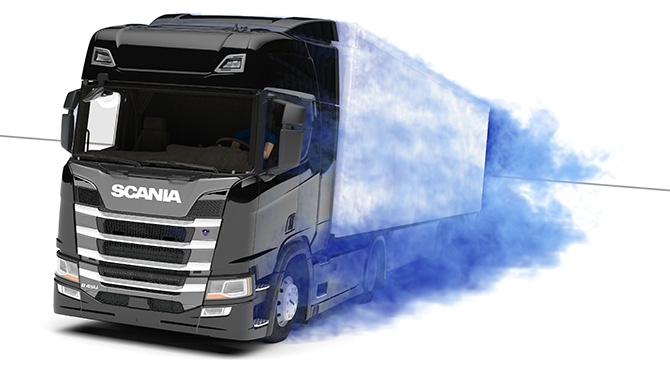
\includegraphics[width=\columnwidth]{Scania_truck}
\column{.5\textwidth}
\footnotesize
PDC's largest industrial partner is Scania. The figure shows a volume rendering of the instantaneous velocity magnitude on the leeward side of a Scania R20 Highline truck at crosswind conditions. (Source: Scania)
\end{columns}
\footnotesize
\begin{itemize}
    \item Businiess partners \\
        \href{https://www.pdc.kth.se/research/business-research/pdc-partners}{https://www.pdc.kth.se/research/business-research/pdc-partners}
    \item White papers from research collaborations between PDC and European companies \\
        \href{https://www.pdc.kth.se/research/business-research/white-papers-1.737818}{https://www.pdc.kth.se/research/business-research/white-papers-1.737818}
\end{itemize}
}

\subsection*{Staff}
\frame{
\frametitle{Support and System Staff}
\begin{exampleblock}{First-line support}
  Provide specific assistance to PDC users related to accounts, login, allocations etc.
\end{exampleblock}
\begin{exampleblock}{System staff}
  System managers/administrators ensure that computing and storage resources run smoothly and securely.
\end{exampleblock}
\begin{exampleblock}{Application Experts}
  Hold PhD degrees in various fields and specialize in HPC. Assist researchers in optimizing, scaling and enhancing scientific codes for current and next generation supercomputers.
\end{exampleblock}
}

\section{Infrastructure}

\subsection{Dardel}
\frame{
\frametitle{Dardel - an HPE Cray XE supercomputer}

\begin{alertblock}{}{\alert{CPU partition}}\end{alertblock}

\begin{columns}
\column{.6\textwidth}
  \begin{itemize}
    \item 2.279 petaFlops (Top500 Nov 2021)
    \item 554 CPU nodes
    \item Dual AMD EPYC$^{\rm TM}$ 64-core processors
    \item 256, 512, 1024, or 2048 GB memory
  \end{itemize}
\column{.4\textwidth}
  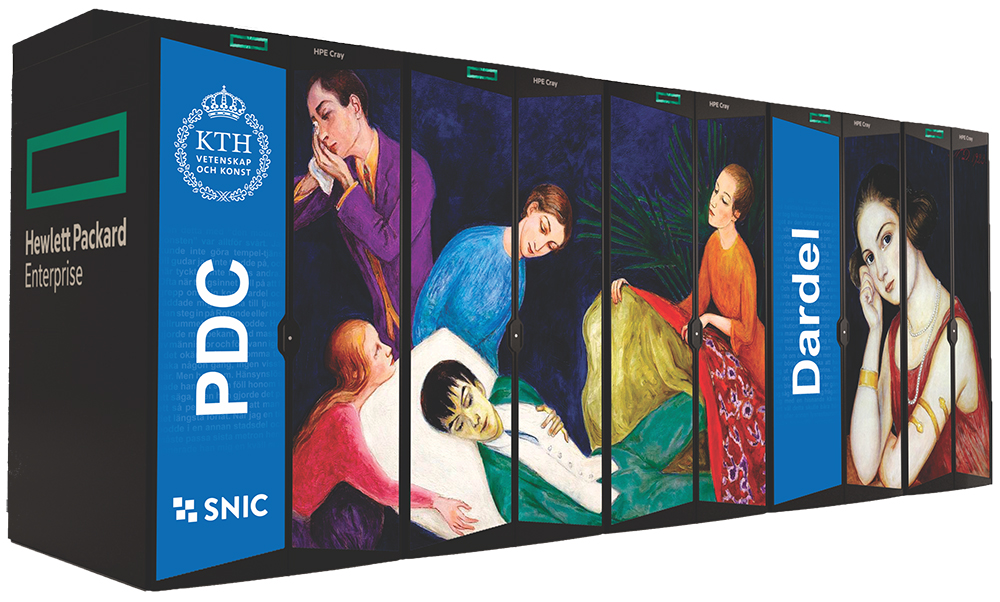
\includegraphics[width=\columnwidth]{dardel}
\end{columns}

\begin{alertblock}{}{\alert{GPU partition}}\end{alertblock}

\begin{columns}
\column{1.\textwidth}
  \begin{itemize}
    \item $56$ GPU nodes
    \item AMD EPYC$^{\rm TM}$ processor with 64 cores (under development)
    \item 512 GB memory
    \item four AMD Instinct$^{\rm TM}$ MI250X GPUs
  \end{itemize}
\end{columns}

}

\subsection*{File systems}
\frame{
\frametitle{File Systems}

\begin{block}{Lustre File System (\alert{Klemming})}
\begin{itemize}
 \item Open-source massively parallel distributed file system
 \item Optimized for handling data from many clients
 \item Total size is $12$ PB (12,000 TB)
 \item Home directory (25 GB, with backup)\\  {/cfs/klemming/home/[u]/[username]}
 \item Project directory \\  {/cfs/klemming/projects/snic/[projectname]}
 \item Scratch directory \\  {/cfs/klemming/scratch/[u]/[username]}
\end{itemize}
\end{block}

\footnotesize
\href{https://www.pdc.kth.se/support/documents/data\_management/klemming.html}{https://www.pdc.kth.se/support/documents/data\_management/klemming.html}

}

\frame{
\frametitle{File Systems}

\begin{itemize}
\item Good practice
    \begin{itemize}
    \item Minimize the number of I/O operations
    \item Avoid creating too many files
    \item Avoid creating directories with a large numbers of files
    \end{itemize}
\end{itemize}

\begin{itemize}
\item Bad practice
    \begin{itemize}
    \item Small reads
    \item Opening many files
    \item Seeking within a file to read a small piece of data
    \end{itemize}
\end{itemize}

}


\begin{frame}[fragile]
\frametitle{Access Control Lists}

\begin{exampleblock}{To view the access for a folder:}
\footnotesize
\begin{verbatim}
getfacl -a /cfs/klemming/home/u/user/test
\end{verbatim}
\end{exampleblock}

\begin{exampleblock}{The output looks like this:}
\footnotesize
\begin{verbatim}
# file: /cfs/klemming/home/u/user/test
# owner: me
# group: users
user::rwx
group::r-x
other::---
\end{verbatim}
\end{exampleblock}

\begin{exampleblock}{To grant the access to another user:}
\footnotesize
\begin{verbatim}
setfacl -m u:<uid>:r-x -R /cfs/klemming/home/u/user/test
\end{verbatim}
\end{exampleblock}

\begin{exampleblock}{To remove the access for another user:}
\footnotesize
\begin{verbatim}
setfacl -x u:<uid> -R /cfs/klemming/home/u/user/test
\end{verbatim}
\end{exampleblock}

\end{frame}



\frame<presentation:0>[noframenumbering]{
\frametitle{File System Access}
 \begin{tabular}{ccc}
   
  \cellcolor{kthLightGreen} \textbf{AFS} & 
  \cellcolor{kthLightBlue}{Beskow Compute Node} &
  \cellcolor{kthLightBlue}\textbf{CFS}\\
   
  \cellcolor{kthLightGreen} Andrew File System & 
  \cellcolor{kthLightGreen!50!kthLightBlue} Beskow Login Node &  
  \cellcolor{kthLightBlue} Lustre File System\\ 
  
  \cellcolor{kthLightGreen}~ &
  \cellcolor{kthLightGreen!50!kthLightBlue}~ &
  \cellcolor{kthLightBlue}~\\

  \cellcolor{kthLightGreen} & 
  \cellcolor{kthLightGreen!50!kthLightBlue} Tegner Compute Node &  
  \cellcolor{kthLightBlue} \scriptsize{\url {/cfs/klemming/ }\alert{\textbf{nobackup}}\url{/}} \\
  
  
  \cellcolor{kthLightGreen} \scriptsize{\url{/afs/pdc.kth.se/home/}} & 
  \cellcolor{kthLightGreen!50!kthLightBlue} Tegner Login Node &  
  \cellcolor{kthLightBlue} \scriptsize{\url{/[initial]/[username]}} \\

  \cellcolor{kthLightGreen} \scriptsize{\url{/[initial]/[username]}}  &
  \cellcolor{kthLightGreen} &
  \cellcolor{kthLightBlue} \\

  \cellcolor{kthLightGreen} & 
  \cellcolor{kthLightGreen} KTH (Linux) computer &  
  \cellcolor{kthLightBlue} \scriptsize{\url{/cfs/klemming/}\alert{\textbf{scratch}}\url{/}}\\
 
  \cellcolor{kthLightGreen} &
  \cellcolor{kthLightGreen} & 
  \cellcolor{kthLightBlue} \scriptsize{\url{/[initial]/[username]}}\\
   
  \cellcolor{kthLightGreen} & 
  \cellcolor{kthLightGreen} Laptop/Home computer &
  \cellcolor{kthLightBlue}
  \end{tabular}
}

\frame<presentation:0>[noframenumbering]{
\frametitle{File System Access}
 
\begin{tikzpicture}
\begin{scope}[transparency group]
\begin{scope}[blend mode=multiply]
  \coordinate (AFS) at (1,0);
  \coordinate (CFS) at (4,0);
  \coordinate (LARGE) at (9,0);
  %\node at (3,-1) {\alert{\textbf{AFS}}}; 
  \node[align=center,text width=3.1cm] at (2.5,1.5) {\textbf{\alert{Tegner Login Node}}};
  \node[align=center,text width=3.1cm] at (2.5,0) {\textbf{Tegner Compute Node}};
  \node[align=center,opacity=1,text width=1.5cm] at (2.5,-2) {\textbf{Beskow Login Node}};
  
  \node[align=center,text width=2cm] at (6,0) {\textbf{Beskow Compute Node}};
  
  \node[align=left,text width=2.3cm] at (0,2) {\textbf{KTH (Linux) computer}};
  \node[align=center,text width=2.5cm] at (-1,-1) {\textbf{Laptop/Home computer}};
  
  \filldraw[fill=kthLightBlue, draw=black,opacity=0.5,rounded corners=1mm] (AFS) \irregularcircle{3.5cm}{3mm};
  \filldraw[fill=kthLightGreen, draw=black,opacity=0.5,rounded corners=1mm] (CFS) \irregularcircle{3.5cm}{2mm};
\end{scope}
\end{scope}
\end{tikzpicture}

  
}

\section{Accounts}

\subsection*{Access requirements}
\frame{
\frametitle{Access requirements}

\begin{description}
\item [User account] either SUPR or PDC
\item [Time allocation] set the access limits
\end{description}

\begin{alertblock}{Apply for PDC account via SUPR}
\begin{itemize}
  \item http://supr.snic.se
  \item SNIC database of persons, projects, project proposals and more
  \item Apply and link SUPR account to PDC
  \item Valid cellphone number for password
\end{itemize}
\end{alertblock}

\begin{alertblock}{Apply for PDC account via PDC}
\begin{itemize}
  \item \href{https://www.pdc.kth.se/support}{https://www.pdc.kth.se/support} $\to$ "Getting Access"
  \item Electronic copy of your passport
  \item Valid cellphone number for password 
  \item Valid reason for applying for account (e.g. attending course)
\end{itemize}
\end{alertblock}

}


\subsection{Authentication}
\begin{frame}[fragile]
\frametitle{Authentication}
\begin{exampleblock}{\large{SSH key pairs}}
\begin{itemize}
  \item Authentication using SSH asymmetric key pairs is very common.
  \item Each SSH key pair includes two keys: a public key and a secret key.
  \begin{itemize}
    \item The public key should be copied to the SSH server. 
    \item The private key must remain with the user and should be kept secret.
  \end{itemize}
  \item PDC implementation
  \begin{itemize}
    \item Only works for Dardel
    \item Restricted by user-defined IPs
    \item SSH keys have to be renewed regularly
  \end{itemize}
\end{itemize}
\end{exampleblock}

\href{https://www.pdc.kth.se/support/documents/login/ssh\_login.html}{https://www.pdc.kth.se/support/documents/login/ssh\_login.html}

\end{frame}

\subsection*{SSH keys}

\begin{frame}[fragile]
\frametitle{Login using SSH keys}

\begin{block}{Create SSH key pairs}
\begin{verbatim}
$ ssh-keygen -t ed25519 -f $HOME/.ssh/id-ed25519-pdc
\end{verbatim}
\end{block}

\begin{block}{Upload your public key in the login portal}
    \begin{itemize}
        \item SUPR authentication for initial setup
        \item PDC login portal for managing/changing user’s connection information (public key and IP address)
        \item See online documentation for details (link below).
    \end{itemize}
\end{block}

\href{https://www.pdc.kth.se/support/documents/login/ssh\_login.html}{https://www.pdc.kth.se/support/documents/login/ssh\_login.html}

\end{frame}


\begin{frame}[fragile]
\frametitle{Configure your SSH}

\begin{block}{\$HOME/.ssh/config}
\begin{verbatim}
... write me ...
\end{verbatim}
\end{block}

\end{frame}

\section{Development}
\subsection{Building}
\begin{frame}[fragile]
\frametitle{Compiling, Linking and Running Applications}
\framesubtitle{on HPC clusters}
 \begin{description}
    \item [source code] C / C++ / Fortran ( \verb|.c, .cpp, .f90, .h|  )
    \item [compile] Cray/GNU/AMD compilers
    \item [assemble] into machine code (object files: \verb|.o, .obj| )
    \item [link] Static Libraries (\verb|.lib, .a|  ) \\ Shared Library (\verb|.dll, .so| ) \\ Executables (\verb|.exe, .x| )
    \item ~ 
    \item [request allocation] submit job request to SLURM queuing system \\ \verb|salloc/sbatch|
    \item [run] application on scheduled resources \\ \verb|srun|
 \end{description}
\end{frame}

\subsection{Modules}
\begin{frame}[fragile]
\frametitle{Modules}
\framesubtitle{Using Lmod}

\begin{exampleblock}{List loaded modules}
  \begin{verbatim}
  ml
  \end{verbatim}
\end{exampleblock}

\begin{exampleblock}{List available modules}
  \begin{verbatim}
  ml avail
  \end{verbatim}
\end{exampleblock}

\begin{exampleblock}{Load modules}
  \begin{verbatim}
  ml <software_name>
  \end{verbatim}
\end{exampleblock}

\begin{exampleblock}{Unload modules}
  \begin{verbatim}
  ml -<software_name>
  \end{verbatim}
\end{exampleblock}
\end{frame}


\begin{frame}[fragile]
\frametitle{Modules }
\framesubtitle{Displaying modules}
\begin{exampleblock}{\$ ml}
\scriptsize
\begin{verbatim}
Currently Loaded Modulefiles:
  1) craype-x86-rome
  ...
  10) cray-libsci/21.08.1.2
\end{verbatim}
\end{exampleblock}

\begin{exampleblock}{\$ ml avail [software\_name]}
\scriptsize
\begin{verbatim}
---------------- /opt/cray/pe/lmod/modulefiles/cpu/x86-rome/1.0 ---------------
     cray-fftw/3.3.8.10    cray-fftw/3.3.8.11    cray-fftw/3.3.8.12 (D)
\end{verbatim}
\end{exampleblock}

\begin{exampleblock}{\$ module show [software\_name]}
\scriptsize
\begin{verbatim}
...
whatis("FFTW 3.3.8.12 - Fastest Fourier Transform in the West")
setenv("FFTW_VERSION","3.3.8.12")
setenv("CRAY_FFTW_VERSION","3.3.8.12")
setenv("FFTW_ROOT","/opt/cray/pe/fftw/3.3.8.12/x86_rome")
...
\end{verbatim}
\end{exampleblock}
\end{frame}

\subsection{Programming environments}
\begin{frame}[fragile]
  \frametitle{Programming Environment Modules}

\begin{columns}[t]
\column{.7\textwidth}
  \begin{description}
  \item [Cray] \verb|$ ml PrgEnv-cray|
  \item [GNU] \verb|$ ml PrgEnv-gnu|
  \item [AMD] \verb|$ ml PrgEnv-aocc|
  \end{description}
   % \item Module cray-libsci provides BLAS, LAPACK, BLACS, and SCALAPACK
   % \item Module cray-mpich provides MPI
\column{.3\textwidth}
    \begin{verbatim}
$ cc	source.c
$ CC	source.cpp
$ ftn	source.F90
  \end{verbatim}
\end{columns}
  \begin{exampleblock}{Compiler wrappers : \alert{\textbf{cc} \textbf{CC} \textbf{ftn}}}
    \alert{Advantages}\\
    Compiler wrappers will automatically 
    \begin{itemize}
      \item link to BLAS, LAPACK, BLACS, SCALAPACK, FFTW\\
      \item use MPI wrappers\\
    \end{itemize}
    \alert{Disadvantage}\\
    Sometimes you need to edit Makefiles which are not designed for Cray 
\end{exampleblock}
\end{frame}


\begin{frame}[fragile]
\frametitle{Programming Environment Modules}
    \begin{exampleblock}{The PDC module}
        .. write me ..
    \end{exampleblock}
\end{frame}

\section{Running jobs}
\frame{
\frametitle{How to run programs}
\begin{itemize}
  \item After login we are on a \textit{login node} used only for:
  \begin{itemize}
    \item submitting jobs,
    \item editing files,
    \item compiling small programs,
    \item other computationally light tasks.
  \end{itemize}
  \item \alert{Never run calculations interactively on the login node} 
  \item Instead, request compute resources \textit{interactively} or via \textit{batch script} \\~

  \item All jobs must be connected to a time allocation
  \item For courses, PDC sets up a \textit{reservation} for resources \\~

  \item To manage the workload on the clusters, PDC uses a queueing/batch system

  \end{itemize}
 }


\subsection{SLURM}
\frame{
\frametitle{SLURM workload manager}
\framesubtitle{Simple Linux Utility for Resource Management}

\begin{itemize}
 \item Open source, fault-tolerant, and highly scalable cluster management and job scheduling system
 \begin{itemize}
  \item \alert{Allocates} exclusive and/or non-exclusive access to \alert{resources} for some duration of time
  \item Provides a framework for \alert{starting}, \alert{executing}, and \alert{monitoring} work on the set of allocated nodes
  \item \alert{Arbitrates contention} for resources by managing a queue 
 \end{itemize}
 \item Job Priority computed based on 
 \begin{description}
    \item [Age] the length of time a job has been waiting
    \item [Fair-share] the difference between the portion of the computing resource that has been promised and the amount of resources that has been consumed
    \item [Job size] the number of nodes or CPUs a job is allocated
    \item [Partition] a factor associated with each node partition
%    \item [QOS] a factor associated with each Quality Of Service
 \end{description}
\end{itemize}
}

\subsection*{SLURM commands}

\begin{frame}[fragile]
\frametitle{Interactive session \hfill \alert{\textbf{salloc}}}

\begin{exampleblock}{Request an interactive allocation of resources}
  \begin{verbatim}
  $ salloc -A <account> -t <d-hh:mm:ss> -N <nodes>
  salloc: Granted job allocation 123456
  \end{verbatim}
\end{exampleblock}

\begin{exampleblock}{Run application on compute nodes}
  \begin{verbatim}
  $ srun -n <PEs> ./binary.x
  #PEs: number of processing elements (MPI processes)
  \end{verbatim}
\end{exampleblock}
  
\end{frame}

\begin{frame}[fragile]
\frametitle{Launch batch jobs \hfill  \alert{\textbf{sbatch}}}
\begin{exampleblock}{Submit the job to SLURM queue}
  \begin{verbatim}
$ sbatch <script>
Submitted batch job 123456
  \end{verbatim}
\end{exampleblock}

\scriptsize
The script should contain all necessary data to identify the account and requested resources 
\begin{exampleblock}{Example of request to run myexe for 1 hour on 2 nodes}
\begin{verbatim}
#!/bin/bash

#SBATCH -A 20XX-X-XX
#SBATCH -J myjob
#SBATCH -t 01:00:00
#SBATCH --nodes=2
#SBATCH --ntasks-per-node=128

srun ./myexe > my_output_file
\end{verbatim}
\end{exampleblock}

\end{frame}

\begin{frame}[fragile]
\frametitle{Monitoring and/or cancelling running jobs }
\begin{alertblock}{\textbf{squeue} -u  \$USER}
  Displays all queue and/or running jobs that belong to the user
\tiny
  \begin{verbatim}
user@dardel$ squeue -u user
 JOBID     USER ACCOUNT           NAME  ST REASON    START_TIME                TIME  TIME_LEFT NODES
 63519   user 20XX-X-XX      test-run1   R None      2021-11-15T08:15:24    6:09:42   17:49:18     2
 63757   user 20XX-X-XX      test-run2   R None      2021-11-15T11:14:20    3:10:46   20:48:14     8
  \end{verbatim}
\end{alertblock}

\begin{alertblock}{\textbf{scancel} [job]}
Stops a running job or removes a pending one from the queue
\tiny
  \begin{verbatim}
user@dardel$ scancel 63519
salloc: Job allocation 63519 has been revoked.

user@dardel$ squeue -u user
 JOBID     USER ACCOUNT           NAME  ST REASON    START_TIME                TIME  TIME_LEFT NODES
 63757   user 20XX-X-XX      test-run2   R None      2021-11-15T11:14:20    3:10:46   20:48:14     8
  \end{verbatim}
\end{alertblock}
\end{frame}

%\fontsize{12pt}{13.2}\selectfont
\section{How to get help}

\subsection*{PDC suppport}
\frame{
\frametitle{PDC support}
\begin{itemize}
  \item Many questions can be answered by reading the web documentation: \alert{\url{https://www.pdc.kth.se/support}}
  \item Preferably contact PDC support by support form:
  \begin{itemize}
    \item If you have SUPR account, use \\
        \alert{\url{https://supr.snic.se/support}}
    \item If you do not have a SUPR account, use \\
        \alert{\url{https://pdc-web.eecs.kth.se/supportStatic/query.html}}
  \end{itemize}
  \item Other ways to contact PDC
    \footnotesize
    \href{https://www.pdc.kth.se/support/documents/contact/contact\_support.html}{https://www.pdc.kth.se/support/documents/contact/contact\_support.html}
\end{itemize}
}

\subsection*{How to report problems}
\frame{
\frametitle{When reporting problems...}
\begin{itemize}
  \item Do not report new problems by replying to old/unrelated tickets.
  \item Be as specific as possible.
  \item Provide necessary information to reproduce the problem.
  \item For problems with scripts/jobs, give an example.
    \begin{itemize}
      \item Make the problem example as small/short as possible.
    \end{itemize}
  \item If you want the PDC support to inspect some files, make sure that the files are readable.
    \begin{itemize}
      \item Do not assume that PDC support personnel have admin rights\\ to see all your files or change permissions.
    \end{itemize}
\end{itemize}
}

\frame{\huge\centering Questions...?}

%\include{live_demo}

\end{document}


